\documentclass[border=5pt]{standalone}
\usepackage[T1]{fontenc}
\usepackage{lmodern,amsmath}
\usepackage[american]{circuitikz}
\usepackage{pgfplots}
\pgfplotsset{compat=1.18}
\usetikzlibrary{arrows.meta}
\begin{document}
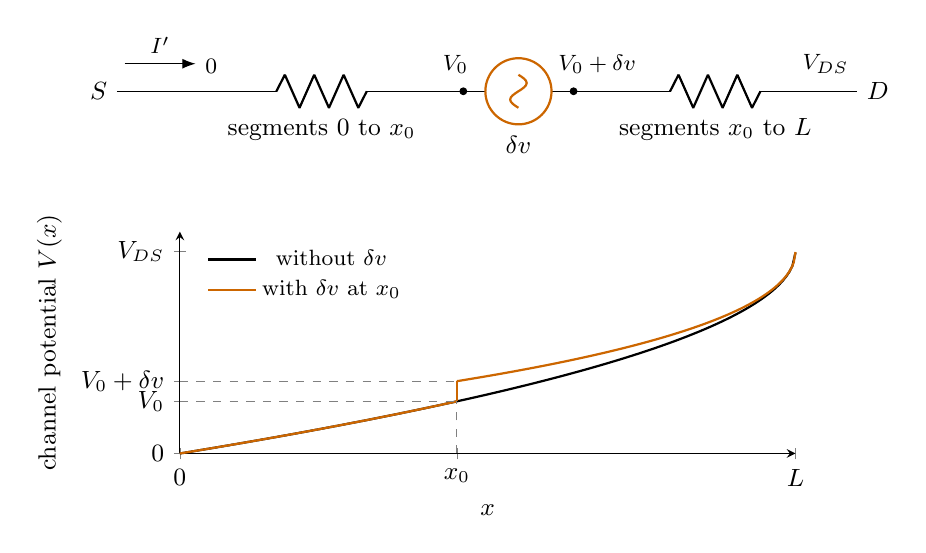
\begin{tikzpicture}[font=\small,>=Latex]
% top: chain with the inserted voltage
\draw (-0.8,0) node[left]{$S$} -- (0.4,0)
  to[R, l_=segments $0$ to $x_0$] (3.2,0) -- (3.6,0)
  to[sV, l_=$\delta v$, color=orange!80!black] (5.0,0) -- (5.4,0)
  to[R, l_=segments $x_0$ to $L$] (8.2,0) -- (8.6,0) node[right]{$D$};
\filldraw (3.6,0) circle (1.2pt); \filldraw (5.0,0) circle (1.2pt);
\node[above,font=\footnotesize] at (0.4,0.1) {$0$};
\node[above,font=\footnotesize] at (3.5,0.1) {$V_0$};
\node[above,font=\footnotesize] at (5.3,0.1) {$V_0+\delta v$};
\node[above,font=\footnotesize] at (8.2,0.1) {$V_{DS}$};
\draw[->] (-0.7,0.35) -- (0.2,0.35) node[midway,above,font=\footnotesize]{$I'$};
% bottom: potential along the channel
\begin{axis}[at={(0,-4.6cm)},anchor=south west,width=9.4cm,height=4.4cm,
  xmin=0,xmax=1,ymin=0,ymax=1.1,
  xtick={0,0.45,1},xticklabels={$0$,$x_0$,$L$},
  ytick={0,0.2584,0.3584,1},yticklabels={$0$,$V_0$,$V_0+\delta v$,$V_{DS}$},
  xlabel={$x$},ylabel={channel potential $V(x)$},
  axis lines=left,samples=200,clip=false,
  legend style={at={(0.03,0.97)},anchor=north west,draw=none,fill=none,font=\footnotesize}]
\addplot[black,thick,domain=0:1] {1-sqrt(1-x)};
\addlegendentry{without $\delta v$}
\addplot[orange!80!black,thick,domain=0:0.45] {1-sqrt(1-x)};
\addlegendentry{with $\delta v$ at $x_0$}
\addplot[orange!80!black,thick,domain=0.45:1] {1-sqrt(1-x)+0.1*(1-x)/(0.55)};
\draw[orange!80!black,thick] (axis cs:0.45,0.2584) -- (axis cs:0.45,0.3584);
\draw[dashed,gray] (axis cs:0,0.2584) -- (axis cs:0.45,0.2584);
\draw[dashed,gray] (axis cs:0,0.3584) -- (axis cs:0.45,0.3584);
\draw[dashed,gray] (axis cs:0.45,0) -- (axis cs:0.45,0.2584);
\end{axis}
\end{tikzpicture}
\end{document}
